\documentclass[10pt]{article}
\usepackage[paperwidth=12cm,paperheight=8.2cm,margin=3mm]{geometry}
\usepackage{tikz}
\pagestyle{empty}
\pagecolor{white}

\begin{document}
\centering
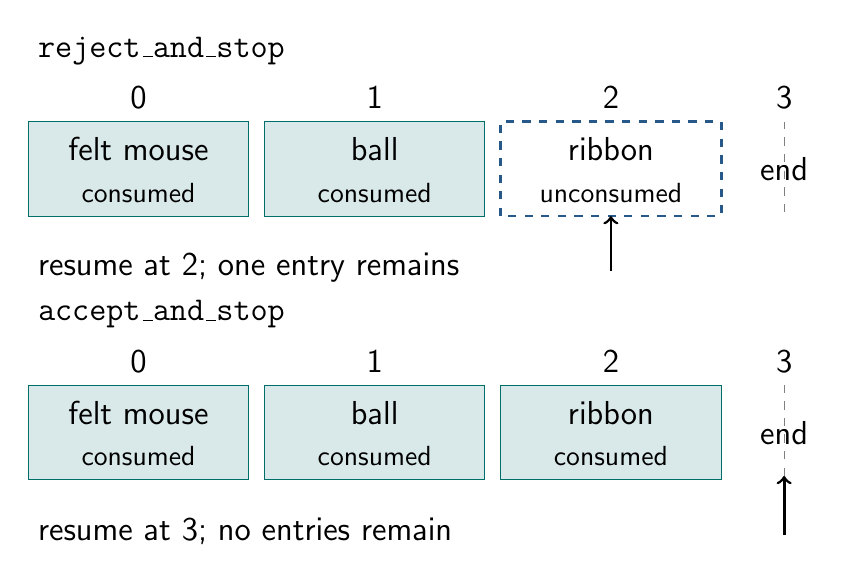
\begin{tikzpicture}[x=1cm,y=1cm,font=\sffamily\large]
  \definecolor{inputcolor}{RGB}{38,89,137}
  \definecolor{resultcolor}{RGB}{0,111,106}

  \node[anchor=west,font=\ttfamily\large] at (0,5.8) {reject\_and\_stop};
  \node[anchor=west,font=\ttfamily\large] at (0,2.45) {accept\_and\_stop};

  \foreach \base in {3.7,0.35} {
    \foreach \offset/\index/\name in {0/0/felt mouse,3/1/ball,6/2/ribbon} {
      \node at (\offset+1.4,\base+1.5) {\index};
      \node at (\offset+1.4,\base+0.85) {\name};
    }
    \node at (9.6,\base+1.5) {3};
    \node at (9.6,\base+0.6) {end};
    \draw[gray,dashed] (9.6,\base+0.05) -- (9.6,\base+1.2);
    \foreach \offset in {0,3} {
      \filldraw[fill=resultcolor!15,draw=resultcolor]
        (\offset,\base) rectangle (\offset+2.8,\base+1.2);
      \node at (\offset+1.4,\base+0.85) {
        \ifnum\offset=0 felt mouse\else ball\fi};
      \node[font=\sffamily\normalsize] at (\offset+1.4,\base+0.3) {consumed};
    }
  }

  \draw[inputcolor,dashed,line width=1pt] (6,3.7) rectangle (8.8,4.9);
  \node[font=\sffamily\normalsize] at (7.4,4.0) {unconsumed};
  \draw[->,line width=1pt] (7.4,3.0) -- (7.4,3.7);
  \node[anchor=west] at (0,3.05) {resume at 2; one entry remains};

  \filldraw[fill=resultcolor!15,draw=resultcolor] (6,0.35) rectangle (8.8,1.55);
  \node at (7.4,1.2) {ribbon};
  \node[font=\sffamily\normalsize] at (7.4,0.65) {consumed};
  \draw[->,line width=1pt] (9.6,-0.35) -- (9.6,0.4);
  \node[anchor=west] at (0,-0.3) {resume at 3; no entries remain};
\end{tikzpicture}
\end{document}
